\section{Results}
\label{sec:results-residual}

\paragraph{Complete-decision quality at the primary budget.}
Table~\ref{tab:main-runtime-ablation} compares \method{} (Capacity), all six
classical priorities, and four matched learned controls. All 15 fits and
24 validation graphs contribute to the 1,512 complete decisions across
three deadlines. Fitting seeds are averaged within each graph before
assigning equal mass to the menu and resource domains. The gain is the
strictly returned improvement relative to the original incumbent, not the
best solution internally available before caller return.

Figure~\ref{fig:online-budget-v4} separates complete return quality,
additional recovery, and caller deadline misses. At the primary
$D=0.556$\,s, Capacity returns 57.542\% gain, while the greedy-only
policy returns the shared prefix's 234.266\% gain in 0.035\,s.
Capacity's 83.333\% late-return rate removes otherwise materialized
improvements from the strict objective. The primary comparison therefore
does not establish a learned-policy advantage; Section~\ref{sec:discussion-residual}
discusses the implications for finite allocation. Longer allowances expose
the additional recovery that a short complete deadline cannot retain.

\begin{table*}[t]
\centering
\caption{\textbf{Complete-decision comparison on all 24 validation graphs.}
Gain: timely improvement over the original incumbent (\%, higher is better).
Late: caller deadline-miss fraction. Time: actual caller latency (s), including
late returns. Aggregation is graph-first and domain-balanced; bold marks the
highest mean at each deadline, without a significance claim.}
\label{tab:main-runtime-ablation}
\footnotesize
\setlength{\tabcolsep}{4pt}
\begin{tabular}{@{}lrrrrrrrrr@{}}
\toprule
& \multicolumn{3}{c}{$D=0.139$\,s} & \multicolumn{3}{c}{$D=0.556$\,s (primary)} & \multicolumn{3}{c}{$D=2.221$\,s} \\
\cmidrule(lr){2-4}\cmidrule(lr){5-7}\cmidrule(lr){8-10}
Method & Gain $\uparrow$ & Late $\downarrow$ & Time $\downarrow$ & Gain $\uparrow$ & Late $\downarrow$ & Time $\downarrow$ & Gain $\uparrow$ & Late $\downarrow$ & Time $\downarrow$ \\
\midrule
\textbf{\method{} (Capacity)} & 74.887 & 0.861 & 0.240 & 57.542 & 0.833 & 0.642 & 236.334 & 0.000 & 1.725 \\
\midrule
AnytimeGreedyPortfolio & \textbf{234.266} & 0.000 & 0.035 & \textbf{234.266} & 0.000 & 0.035 & 234.266 & 0.000 & 0.035 \\
Immediate & 21.107 & 0.944 & 0.232 & 21.107 & 0.944 & 0.634 & 234.624 & 0.000 & 1.429 \\
Upper & 108.040 & 0.778 & 0.218 & 43.078 & 0.889 & 0.642 & 234.266 & 0.000 & 1.606 \\
PairPriority (P1) & 78.310 & 0.861 & 0.230 & 56.909 & 0.889 & 0.648 & 236.218 & 0.000 & 1.474 \\
Lower & 21.107 & 0.944 & 0.234 & 0.000 & 1.000 & 0.651 & 234.393 & 0.000 & 1.602 \\
RoundRobin & 21.107 & 0.944 & 0.231 & 13.348 & 0.972 & 0.636 & 234.266 & 0.000 & 1.480 \\
\midrule
FreeOccupancy & 76.759 & 0.861 & 0.240 & 43.099 & 0.889 & 0.650 & 237.007 & 0.000 & 1.696 \\
NoAux & 80.406 & 0.852 & 0.240 & 51.799 & 0.843 & 0.642 & 236.916 & 0.000 & 1.726 \\
NoWarm & 71.939 & 0.870 & 0.238 & 69.318 & 0.833 & 0.642 & 236.891 & 0.000 & 1.721 \\
CheapSummary & 73.834 & 0.861 & 0.230 & 94.665 & 0.806 & 0.645 & \textbf{238.355} & 0.000 & 1.674 \\
\bottomrule
\end{tabular}
\par\smallskip
\begin{minipage}{\textwidth}
\footnotesize
All methods share the executed greedy prefix; every native request uses
the CHILS-p1 recovery kernel~\cite{grossmann2025chils}. Upper uses the classical clique
bound~\cite{chvatal1975polytopes}. These are matched allocation controls,
not separate published whole-graph solvers. All graph and fit slots retain
their prescribed weights; a late final return receives zero strict gain.
Once-only resident graph/model setup is excluded from decision time.
\end{minipage}
\end{table*}

\begin{figure*}[t]
\centering
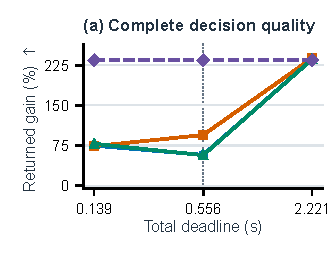
\includegraphics[width=0.326\textwidth]{v4_figures/residual_results/online_quality.pdf}\hfill
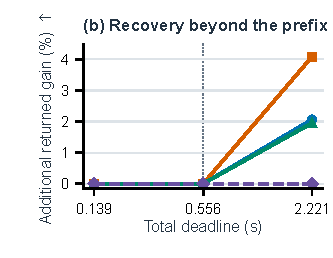
\includegraphics[width=0.326\textwidth]{v4_figures/residual_results/online_extra.pdf}\hfill
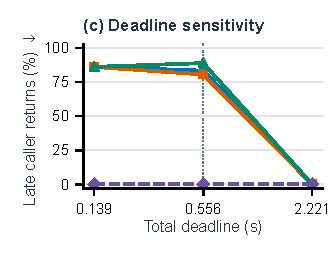
\includegraphics[width=0.326\textwidth]{v4_figures/residual_results/online_lateness.pdf}\\

\includegraphics[width=0.94\textwidth]{v4_figures/residual_results/online_legend.pdf}
\caption{\textbf{Joint recovery under complete decision budgets.}
All 1,512 runs use graph-first, equal-domain aggregation.
(a) Validated gain actually received before the deadline.
(b) Additional gain beyond the paid common prefix.
(c) Caller deadline misses, retaining the original schedule in (a).
Dotted lines mark the primary deadline. Longer budgets admit extra recovery;
CheapSummary remains competitive with the structural predictor.}
\label{fig:online-budget-v4}
\end{figure*}


\paragraph{Longer budgets and matched components.}
At $D=2.221$\,s, all methods return on time. Capacity reaches 236.334\%,
including 2.068 percentage points beyond the 234.266\% common prefix.
The menu and resource contributions above their respective prefixes are
3.882 and 0.254 points. Thus most total improvement still comes from
executed greedy preparation, and the remaining recovery is concentrated
in the menu domain. Percentages exceeding 100\% reflect the original
incumbent denominator; they are neither optimality gaps nor improvements
over the greedy response.

Capacity exceeds PairPriority (P1), the strongest long-budget classical
priority, by only 0.116 points (236.218\% for P1), below the predefined
0.5-point mean materiality criterion. It also requires 1.725\,s mean
caller time versus P1's 1.474\,s. CheapSummary achieves the highest mean
gain, 238.355\%, with 4.090 points above the prefix and 1.674\,s mean
latency. FreeOccupancy, NoAux and NoWarm also exceed Capacity at this
workpoint. These controls retain the same actual warm starts and bounds;
their results provide no consistent online benefit from occupancy
contraction, auxiliary membership supervision, or warm identity. In
particular, the structural encoder does not outperform the scalar summary
control. The representation expresses joint compatibility, but that
mechanism alone is insufficient to establish better finite allocation.

\paragraph{Available recovery and its execution scale.}
Figure~\ref{fig:conditional-recovery-opportunity} explains why additional
recovery is a meaningful, domain-dependent target despite the online
result. Across the complete 72 training and 24 validation graphs, two
fixed execution snapshots retain all zero-opportunity cases. Validation
best single admitted extra averages 20.494\% of original incumbent value:
39.981\% for menus and 1.006\% for resource graphs. Renormalization by
each snapshot's current feasible best yields 7.178\% and 0.848\%,
respectively. Menu incumbents initially contain eight vertices, whereas
the executed prefix selects 49--103, explaining part of the denominator
effect without eliminating residual opportunity.

The 10\,ms workpoint produces no additional global gain; its procedure
usually retains the actual warm recovery. At 50/200\,ms, validation menu
opportunity is 39.061\%/39.981\%, while resource opportunity stays at
1.006\%. Longer search adds best-one opportunity on five of eighteen menu
graphs and none of six resource graphs. The structure panel further shows
that clique-bound headroom can exceed finite feasible recovery. These
conditional single-call outcomes motivate execution-aligned supervision;
they neither certify an adaptive-policy upper bound nor demonstrate that
the learned controller selects or returns those opportunities.

\begin{figure*}[t]
\centering
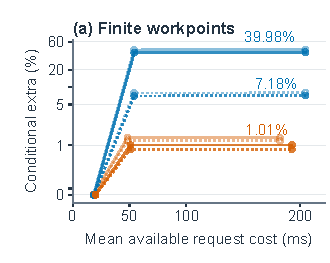
\includegraphics[width=.326\textwidth]{v4_figures/residual_results/opportunity_workpoints.pdf}\hfill
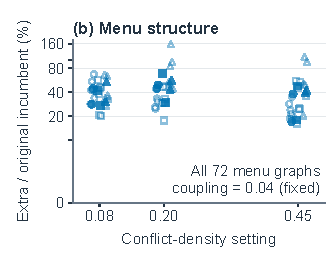
\includegraphics[width=.326\textwidth]{v4_figures/residual_results/opportunity_scenarios.pdf}\hfill
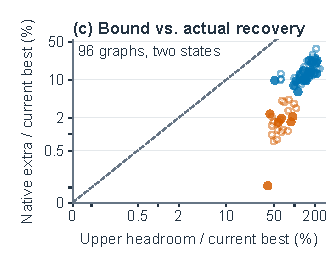
\includegraphics[width=.326\textwidth]{v4_figures/residual_results/opportunity_slack.pdf}

\includegraphics[width=.97\textwidth]{v4_figures/residual_results/opportunity_legend.pdf}
\caption{\textbf{Where additional joint recovery is available.}
Two actual snapshots per development graph.
(a) Best single-call admitted extra versus mean request cost; solid/dotted
curves normalize by original/current incumbents. (b) Menu topology and
density at fixed coupling 0.04. (c) Finite extra versus clique-bound headroom,
normalized by current best; diagonal: equality. Axes are linear near zero,
logarithmic beyond. These are conditional opportunities, not policy gains.}
\label{fig:conditional-recovery-opportunity}
\end{figure*}


\paragraph{Published whole-graph solver profiles.}
Table~\ref{tab:public-published-performance} retains all 17 published
configurations on 40 original public unit-weight graphs. Three runs are
averaged within each graph before equal-family aggregation. All 2,040
runs contribute, including 162 failed returns that preserve the initial
schedule. CHILS-p1 achieves 24.300\%/24.468\% accepted gain at the two
soft workpoints; the separate 16-thread configuration reaches
25.096\%/25.110\%. DIFUSCO's four-sample recipe improves accepted gain
over its one-sample recipe (12.313\% versus 8.724\%), with higher resident
request cost. COExpander's 6.347\% gain accompanies a 0.073\,s resident
cost. These observations characterize solver quality and cost on the
exposed inputs.

Native costs include startup, preprocessing, parsing and validation;
0.5/2\,s search allowances are not complete deadlines. Neural request
costs exclude the separately reported once-only setup. Released SAT-model
training overlap remains unresolved. No complete matched \method{} public
evaluation accompanies these profiles, so they do not establish its
transfer superiority or a speedup under matched total budgets.

\begin{table*}[t]
\centering
\caption{\textbf{Published whole-graph performance on 40 original public graphs.}
Three common initial schedules per graph; accepted gain is relative to the
original incumbent, with failures retaining its weight. Aggregation is
graph-first and family-balanced. Native cold costs and neural resident costs
have different boundaries.}
\label{tab:public-published-performance}
\footnotesize
\setlength{\tabcolsep}{5pt}
\begin{tabular}{@{}llrrrrrr@{}}
\toprule
& & \multicolumn{4}{c}{Accepted gain (\%) $\uparrow$} & & \\
\cmidrule(lr){3-6}
Method & Workpoint & DIMACS & UF & CBS & \textbf{Equal-family} & Cost (s) $\downarrow$ & Valid/120 $\uparrow$ \\
\midrule
\multicolumn{8}{@{}l}{\textbf{Native CPU: one thread; complete cold wall cost}} \\
CHILS-p1~\cite{grossmann2025chils} & 0.5\,s & 56.789 & 7.932 & 8.178 & 24.300 & 0.5455 & 120/120 \\
CHILS-p1~\cite{grossmann2025chils} & 2\,s & 57.235 & 7.961 & 8.209 & 24.468 & 2.0438 & 120/120 \\
$m^2$wis~\cite{grossmann2024mwis} & 0.5\,s & 25.428 & 7.383 & 7.833 & 13.548 & 4.1856 & 93/120 \\
$m^2$wis~\cite{grossmann2024mwis} & 2\,s & 25.428 & 7.383 & 7.833 & 13.548 & 5.5979 & 93/120 \\
$m^2$wis+s~\cite{grossmann2024mwis} & 0.5\,s & 25.428 & 7.162 & 7.491 & 13.360 & 4.1731 & 93/120 \\
$m^2$wis+s~\cite{grossmann2024mwis} & 2\,s & 25.428 & 6.967 & 7.566 & 13.320 & 5.5732 & 93/120 \\
Struction-fast~\cite{gellner2021struction} & 0.5\,s & 25.367 & 1.557 & 2.418 & 9.781 & 0.5519 & 120/120 \\
Struction-fast~\cite{gellner2021struction} & 2\,s & 36.260 & 1.915 & 2.645 & 13.607 & 2.0483 & 120/120 \\
Struction-strong~\cite{gellner2021struction} & 0.5\,s & 25.896 & 1.557 & 2.418 & 9.957 & 0.5482 & 120/120 \\
Struction-strong~\cite{gellner2021struction} & 2\,s & 36.177 & 1.924 & 2.645 & 13.582 & 2.0481 & 120/120 \\
WeightedBR (original)~\cite{lamm2019exact} & 0.5\,s & 13.376 & 4.975 & 6.147 & 8.166 & 3.8401 & 93/120 \\
WeightedBR (original)~\cite{lamm2019exact} & 2\,s & 13.902 & 6.723 & 7.686 & 9.437 & 5.2060 & 93/120 \\
\midrule
\multicolumn{8}{@{}l}{\textbf{Native CPU: 16 threads; complete cold wall cost}} \\
CHILS-p16-c16~\cite{grossmann2025chils} & 0.5\,s & 58.738 & 8.085 & 8.463 & 25.096 & 0.5505 & 120/120 \\
CHILS-p16-c16~\cite{grossmann2025chils} & 2\,s & 58.738 & 8.113 & 8.478 & 25.110 & 2.0494 & 120/120 \\
\midrule
\multicolumn{8}{@{}l}{\textbf{Released neural models: GPU; resident request cost}} \\
DIFUSCO-SAT~\cite{sun2023difusco} & $50\!\times\!1$ & 10.220 & 7.864 & 8.090 & 8.724 & 1.4209 & 120/120 \\
DIFUSCO-SAT~\cite{sun2023difusco} & $50\!\times\!4$ & 20.835 & 7.923 & 8.180 & 12.313 & 5.5737 & 120/120 \\
COExpander-SAT-CM~\cite{ma2025coexpander} & $1\!\times\!1$ & 7.553 & 5.644 & 5.844 & 6.347 & 0.0730 & 120/120 \\
\bottomrule
\end{tabular}
\par\smallskip
\begin{minipage}{\textwidth}
\footnotesize
Native workpoints are soft search allowances, not complete decision deadlines;
cold cost includes export, startup, preprocessing, parsing and validation.
Neural workpoints give steps $\times$ samples (DIFUSCO) or the released CM recipe
(COExpander). Once-only parent setup, excluded from resident cost:
DIFUSCO one/four samples: 5.948/5.946\,s; COExpander: 7.238\,s.
Costs are graph-first, equal-family means; valid counts retain all 120 runs.
\end{minipage}
\end{table*}

